\documentclass[border=2pt]{standalone}
\usepackage{tikz}
\usetikzlibrary{arrows.meta,positioning,shapes.symbols}
\begin{document}
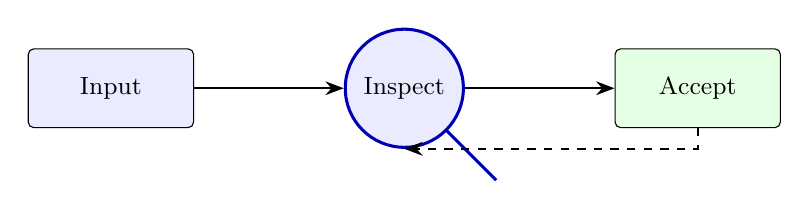
\begin{tikzpicture}[>=Stealth,node distance=19mm,every node/.style={font=\small},
  stage/.style={draw,rounded corners=2pt,minimum width=21mm,minimum height=10mm},
  flow/.style={->,thick}]
  \node[stage,fill=blue!8] (input) {Input};
  \node[magnifying glass,draw=blue!70!black,fill=blue!8,line width=1.1pt,
    minimum size=15mm,magnifying glass handle angle=-45,
    magnifying glass handle aspect=1.2,right=of input] (inspect) {Inspect};
  \node[stage,fill=green!10,right=of inspect] (accept) {Accept};
  \draw[flow] (input.east) -- (inspect.west);
  \draw[flow] (inspect.east) -- (accept.west);
  \draw[flow,dashed] (accept.south) |- (inspect.south);
\end{tikzpicture}
\end{document}
